\documentclass[8pt]{extarticle}
\usepackage{graphicx}
\usepackage[margin=.5in]{geometry}
\usepackage{multicol}
\usepackage{helvet}
\usepackage{algorithm}
\usepackage[noend]{algpseudocode}

\begin{document}
	
	\twocolumn
	
	\title{Controller Assignment}
	\author{Shadman Protik\\Talha Ibn Aziz }
	\date{21/3/2018}
	\maketitle
	
	\section{Existing Algorithms}
	
	We worked with two well-known existing clustering algorithms DBCP (Density Based Controller Placement) and SPICi ('spicy', Speed and Performance In Clustering):
	
	\subsection{Algorithm 1: DBCP}

	DBCP (Density Based Controller Placement) clusters a network using the local density of a node. The local density of a node $s$ is the count of all the nodes which are at most $d_c$ distance away from $s$ and is denoted by $\rho_s$. The threshold $d_c$ is a distance used to set a limit to the cluster diameter and $d_{ij}$ gives the minimum distance between nodes $i$ and $j$.
	\begin{equation}
	\rho_i=\sum_j\chi(d_{ij}-d_c)
	\end{equation}
	
	The value of $\chi(x)$ is 1 only for $d_{ij}>d_c$ that is when $x>0$ and is 0 otherwise. Thus $\rho_i$ is the number of nodes that can be reached from node $i$ by traversing at most distance $d_c$.
	
	The minimum distance to a higher density node is represented by the term $\delta_s$ for a node $s$. For the node with highest density there is no node with higher density. Therefore only for that node, $\delta_s$ holds the distance of the farthest node from $s$.
	
	For a set of nodes $S$ with a set of edges $L$ among them in a graph $G=(S,L)$ they fixed a value of $k$, that is the number of clusters to be formed each with one controller. They formed the clusters and selected a node as controller based on the values of $\rho_s$ and $\delta_s$. The more the values $\rho_s$ and $\delta_s$ for a node $s$, the more it's chances are for being selected as the controller. The method for selecting the cluster head or controller of each sub-network is explained further in detail in the section \ref{perfm}.
	
	\begin{algorithm}
		\caption{: Density Based Controller Placement}\label{euclid}
		\begin{algorithmic}[1]
			\Procedure{DBCP}{S,L} \\
			$k \gets 0$ \\
			\textbf{for $s$ in S:}
			\State $\rho_s=\sum_{j\in S}\chi(d_{sj}-d_c)$ \\
			\textbf{end for} \\
			\textbf{for $s$ in S:}
			\State $\delta_s=\min_{i:i\in S,p_i>p_s}(d_{is})$ \\
			\textbf{end for} \\
			$\delta \gets \frac{1}{|S|}\sum_{s\in S}\delta_s$ \\
			\textbf{for s in S:}
			\If {$\delta_s>\delta$}	
				\State $k = k + 1$
				\State $s \gets newcluster$
			\Else
				\State $s \gets cluster of nearest higher density$
			\EndIf \\
			\textbf{end for}
			\EndProcedure
		\end{algorithmic}
	\end{algorithm}
	
	
	\subsection{Algorithm 2: SPICi}
	
	SPICi ('spicy', Speed and Performance In Clustering) clusters a connected undirected graph $G=(V,E)$ with edges that have confidence values of the continuous range $(0,1)$ so that each cluster has a seed as center from which clustering starts. These edges can be represented by $w_{u,v}$ such that $u,v\in V$, $w_{u,v}\in E$ and $0\le w_{u,v}\le1$. It works with three variables and two thresholds. The three variables can be defined as the weighted degree of a node $d_w$, the density of a set of nodes $S$ and the support of a node $u\in V$ with respect to a set of nodes $S$:
	\begin{equation}
	d_w(u)_{u\in V} = \sum_{v:v\in V,(u,v) \in E}w_{u,v}
	\end{equation}
	
	Therefore $d_w(u)_{u\in V}$ is the sum of all the weights of the edges that connect $u$ with any other adjacent node $v$ of the graph $G=(V,E)$.
	
	\begin{equation}
	density(S) = \frac{\sum_{(u,v)\in E}w_{u,v}}{|S|*(|S|-1)/2} 
	\end{equation}
	
	In other words, $density(S)$ is the sum of the edges that connect every node $u$ with every other node $v$ of $S$ divided by the number of total possible nodes that is $|S|*(|S|-1)/2$ where $|S|$ is the number of nodes present in the set of nodes $S$.
	
	\begin{equation}
	support(u,S) = \sum_{v\in S} w_{u,v}
	\end{equation}
	And $support(u,S)$ is the sum of the edges that connect a node $u$ with the nodes adjacent to it present in the set of nodes $S$.
	
	The thresholds are: $T_s$ which determines whether a node is to be included in the cluster based on the cluster size and the connectivity of the node to the cluster and :$T_d$ which includes a node to the cluster based on the density increased when the node is added.
	\begin{algorithm}
		\caption{: SPICi}\label{euclid}
		\begin{algorithmic}[1]
			\Procedure{Search}{V,E} \\
			\textbf{Initialize} $DegreeQ = V$ \\
			\textbf{While} $DegreeQ \neq empty$
			\State Extract u from DegreeQ with largest $d_w(u)$
			\If {there is $v_{v:v,u\in E}\in DegreeQ$}
			\State $v \gets secondseed(DegreeQ,E,u)$
			\If {$v\neq null$} $S \gets Expand(u,v)$
			\EndIf
			\Else 
				\State $S \gets \{u\}$
			\EndIf
			\State $V \gets V - S $
			\State $Degree Q \gets Degree Q - S$
			\State $d_w(t)_{t:t\in DegreeQ,(t,s)_{s\in S}\in E} = d_w(t) - support(t,S)$
			\EndProcedure\\
			\Procedure{SecondSeed}{V,E,u} \\
			$bin[i]_{i:i=(1,5)} \gets s_{s:s\in V,(s,u)\in E}$ \\
			\textbf{for i = 1 to 5}
			\If {$bin[i] \neq empty$}
				\State \Return $v$ \textbf{if} $d_w(v)=\max_{s:s\in bin[i]}{d_w(s)}$
			\EndIf\\
			\Return $null$
			\EndProcedure\\
			\Procedure{Expand}{V,E,u,v}\\
			\textbf{Initialize} the cluster $S \gets \{u,v\}$ \\
			\textbf{Initialize} $CandidateQ = S_{S:s\in S,(s,u),(s,v)\in E}$\\
			\textbf{While} $CandidateQ \neq empty$
			\State Extract $t$ from Candidate with highest $support(t,S)$
			\If {$support(t,S)\geq T_s*|S|∗density(S)$ and
				$density(S + t)> T_d$}
				\State $S\gets S+\{t\}$
				\State $CanditateQ \gets CandidateQ + \{s_{s:(s,t)\in E}\}$
				\State $CandidateQ \gets CandidateQ - \{s_{s:s\not\in CandidateQ}\}$
				\Else
				\State break from loop
				\EndIf \\
				\Return S
			\EndProcedure
		\end{algorithmic}
	\end{algorithm}
	The nodes are added to bins 1,2,3,4 and 5 respectively if their connected edge value $w_{s,u}\leq0.2,0.3,0.4$ and $0.5$ such that $s,u\in V$ and $(s,u)\in E$.
	
	\section{Proposed Algorithms}
	\subsection{Proposed 1: Modified DBCP}
	
	DBCP considers that the graph is unweighted and ignores the weights even if they are present and uses hop count as a metric to find density using a threshold $d_c$. Modified DBCP does the same thing except that it finds the distances and densities using the weighted edge lengths and the threshold value is also assigned accordingly. It's shortcomings are as follows:
	
	\begin{itemize}
		\item DBCP increases the value of k that is the number of clusters, each time the nearest higher density distance ($\delta_s$) is greater than the average value ($\delta$). If a group of nodes is far away with lower density and nearer nodes have equal density, for each node k increases needlessly when only 1 increase was enough and a cluster was created using nearby nodes. This can be improved by changing the k increase condition.
		\item In case of some networks all nodes have $\rho_s=\rho$ and thus k remains at 0. This is impossible as at least one controller is required for a Software Defined Network. An example graph is given in figure \ref{fig:problem}. In this graph node 1 and 4 have $\rho_s=2$, 2 and 3 have $\rho_s=3$ and so $\delta_s$ for all nodes is 1. Therefore $\rho$ is also 1 and $\rho_s>\rho$ will always be false and k will not be increased. Giving zero clusters which is impossible.
	\end{itemize}

	\begin{figure}
		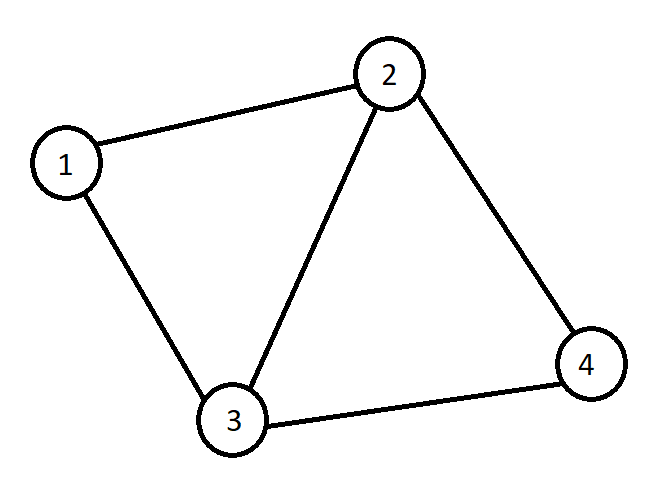
\includegraphics[width=\linewidth]{problem.png}
		\caption{Problematic Graph with edge=1}
		\label{fig:problem}
	\end{figure}
	
	\subsection{Proposed 2: Greedy-SPICi}
	
	This algorithm is identical to SPICi except that it converts all the edges to less than 1 and omits the bin formation. It directly selects the node with maximum weighted degree as second seed. Therefore technically only the second seed selection function changes as given below:
	\begin{algorithm}
		\caption{:Greedy-SPICi Edited Snippet}\label{euclid}
		\begin{algorithmic}[1]
			\Procedure{SecondSeed}{V,E,u} \\
			\Return $v$ \textbf{if} $d_w(v)=\max_{s:(s,u)\in E}{d_w(s)}$
			\EndProcedure
		\end{algorithmic}
	\end{algorithm}

	There are some Shortcomings of this algorithm. These are:
	\begin{itemize}
		\item It considers support and weighted degree as basis for seed selection and cluster choosing parameters thus for greater distances it erroneously thinks the farther node is a better choice as it has higher weighted degree due to incident edges having grater confidence values.
		\item In case of closely connected nodes it creates small clusters due to setting a limit for taking nodes into the clusters. Thus many isolated clusters are created and thus many controllers unnecessarily, which is not ideal for a network.
	\end{itemize}
	\subsection{Proposed 3: Modified-SPICi v2}
	
	This algorithm is the same as SPICi with a few modifications. These are as follows:
	\begin{itemize}
		\item It takes the node with less number of edge as the first seed so that the leaf nodes are selected as starters of clusters.
		\item Post Processing is added. Nodes of cluster will be added to other closest cluster if the cluster size is less then a certain threshold value.
	\end{itemize}
	The change in pseudo-code can be observed to better understand the change and effects that it might cause.
	\begin{algorithm}
		\caption{: Modified SPICi Version 2 Snippet}\label{euclid}
		\begin{algorithmic}[1]
			\Procedure{Search}{V,E} \\
			\textbf{Initialize} $DegreeQ = V$ \\
			\textbf{While} $DegreeQ \neq empty$
			\State \textbf{Extract u from $DegreeQ$ with least edges}
			\If {there is $v_{v:v,u\in E}\in DegreeQ$}
			\State $v \gets secondseed(DegreeQ,E,u)$
			\If {$v\neq null$} $S \gets Expand(u,v)$
			\EndIf
			\Else 
			\State $S \gets \{u\}$
			\EndIf
			\State $V \gets V - S $
			\State $Degree Q \gets Degree Q - S$
			\State $d_w(t)_{t:t\in DegreeQ,(t,s)_{s\in S}\in E} = d_w(t) - support(t,S)$
			\EndProcedure
			\Procedure{Post-Processing}{V,E}\\
				\textbf{for each unclustered s in V:}
					\If{$|S|_{adjacent cluster}<threshold$}
					\State add s to adjacent cluster
					\EndIf \\
				\textbf{end loop}
			\EndProcedure
		\end{algorithmic}
	\end{algorithm}
	\subsection{Proposed 4: Modified-SPICi v3}
	
	The algorithm is the same as SPICi with some modifications. Previously the first seed was selected as the cluster head. In this version a new cluster head selection is used. The modifications are mentioned below:
	\begin{itemize}
		\item Same changes as Modified  V2.
		\item Cluster head selection function is changed. The head will be the node from which the sum of distances to all nodes in that cluster is minimum.
	\end{itemize}

	Thus the Modified-SPICi v3 uses a new function for cluster head selection.
	\begin{algorithm}
		\caption{: Modified SPICi Version 3 Snippet}\label{euclid}
		\begin{algorithmic}[1]
			\Procedure{Head-Selection}{V,E} \\
				\textbf{for each node $s$ in cluster $S$}
				\If {$support(s,S) = \max_{u:u\in S}(support(u,S))$}
				\State $s \gets clusterhead$
				\EndIf \\
				\textbf{end loop}
			\EndProcedure
		\end{algorithmic}
	\end{algorithm}
	
	This change gives a better selection of cluster head for a cluster. As each cluster head should be connected to most number of nodes and thus have a higher support value.
	\subsection{Proposed 5: Modified-SPICi v4}
	
	This algorithm is same as SPICi except for a few changes which make it almost identical to SPICi v3. It's modifications are:
	\begin{itemize}
		\item Same as Modified-SPICi v2.
		\item Cluster head selection function is changed. The head will be the node from which the max of distances to all nodes in that cluster is minimum.
	\end{itemize}	
	
	The changes can be depicted in terms of pseudo-code and thus is shown below:
	\begin{algorithm}
		\caption{: Modified SPICi Version 4 Snippet}\label{euclid}
		\begin{algorithmic}[1]
			\Procedure{Head-Selection}{V,E} \\
			\textbf{for each node $s$ in cluster $S$}
			\If {$\max_{j:j\in S}(d_{sj}) = \min_{i:i\in S}(\max_{j:j\in S}(d_{ij}))$}
			\State $s \gets clusterhead$
			\EndIf \\
			\textbf{end loop}
			\EndProcedure
		\end{algorithmic}
	\end{algorithm}

	In the given pseudo-code snippet above $d_{ij}$ indicates the distance between nodes i and j.
	
	\subsection{Proposed 5: Inverse-SPICi}
	
	This algorithm is taken from SPICi without any post processing or modification except that the cost is taken in an inverse manner. If the graph is represented by $G=(V,E)$ where $V$ is the set of nodes and $E$ is the set of edges containing edge costs $w_{u,v}$ such that $u,v\in V$ and $(u,v)\in E$ the costs can be expressed by the following equations.
	\begin{equation}
	max\_cost = \max_{u,v\in E}(w_{u,v}+1)
	\end{equation}
	\begin{equation}
	cost_{u,v} = max\_cost - w_{u,v}
	\end{equation}
	
	This cost acts as the new edge value when calculating the values of weighted degree, support and density of the required set of nodes.
	
	\section{Thresholds $T_c$ and $d_c$}
	In SPICi the value of Tc have an effect on the cluster size. The Greater the value, less number of nodes there are in a cluster. The value was originally set to 0.5 in SPICi.
	But as we experimented more, we think the value depends more on the type of input graph rather than being a fixed value. For the versions of greedy SPICi we tried to take the value near 0.5.
	
	For Inverse-SPICi when the value is near 1 it gives better results. Slight variation in the value may change the cluster size dramatically. 
	
	\textbf{Problem:} Determining the value of $T_c$
	
	
	\textbf{Solution:} We can do a Binary/Ternary search.
	
	\textbf{Procedure:} 
	\begin{enumerate}
		\item First We will select a value of K (The number of cluster). We won't have more than K clusters.
		\item Perform a Search to determine the value of $T_c$ depending on the result that SPICi gives. We can find a suitable metric for this.
	\end{enumerate}
	 
	\section{Performance Evaluation}
	
	Initially we defined the metrics that we used to evaluate the performance of the algorithms. Then we compared the algorithms using those metrics.
	
	\subsection{Performance Metrics} \label{perfm}
	
	To evaluate the performance of the existing algorithms and the proposed algorithms, we used a number of metrics to define how well an algorithm is compared to another. We defined most of the metrics based on the cluster head selection parameters of the algorithm DBCP.
	After clustering the network they selected the cluster head using a metric which is the sum of three variables.
	
	\subsubsection{Controller-to-switch latency}
	For a sub-network graph, the average propagation latency for
	the placement location v of controller θ is calculated as:
	\begin{equation}
	\pi_{avglatency}(S(\theta)) = min_{v\in S(\theta)} \frac{1}{|S(\theta)|} \sum_{s\in S(\theta)}d(v,s)
	\end{equation}
	
	Here is $S(\theta)$ is the sub-network graph where $\theta$ is the controller of that graph. And $d(v,s)$ is the latency from controller $v$ to switch $s$. The controller is selected so that the average of it's distance from all other nodes in that sub-network is minimized.
	
	Two important factors are $k$ and $max(|S|)$. The lesser value of $k$ the lesser the cost of installing controller and $max(|S|)$ is the maximum number of switches assigned to a controller which gives an idea of the maximum nodes a controller needs to handle.
	
	\begin{center}
		\emph{k = number of clusters or controllers}
	\end{center}
	The value of k is the number of clusters that is to be formed or is formed by the algorithm.
	
	$\pi^{md}(S)$ is the max latency of a node which is basically the maximum distance of each cluster head to other nodes in the cluster S. And $\pi^{md}$ is the max of $\pi^{md}(S)$ for all clusters in the graph.
	\begin{equation}
	\pi^{md}(S)=\max_{j:j\in S}(d_{s,j})
	\end{equation}
	\begin{equation}
	\pi^{md}=\max_{S:S\in G}(\pi^{md}(S))
	\end{equation}
	
	Here $S$ is the set of nodes in a cluster and $s$ is the cluster head of that cluster. G is the graph of the total network.
	
	We used another variable $\pi^{avgd}$ which is the average of the distances of the cluster heads to all the nodes of that cluster.
	
	\begin{equation}
	\pi^{avgd}=\frac{\sum_{S\in G}(\sum_{j:j\in S}(d_{sj}))}{|V|-k}
	\end{equation}
	
	Here $d_{sj}$ represents the minimum distance between nodes $s$ and $j$ where $s$ is the cluster head of the cluster $S$. The total number of nodes is $|V|$ and there are $k$ clusters. So if there are $k$ heads then without these heads each head has a total of $|V|-k$ switches under them. Therefore the total sum of all the distances of the heads to their switches is divided by the total number of switches.
	
	And $\pi^{ic}$ is another metric which represents the average inter-controller distance of a network.
	
	\begin{equation}
	\pi^{ic}=\frac{\sum_{i,j\in H}(d_{ij})}{k*(k-1)/2}
	\end{equation}
	
	Here $H$ is the set of controllers or cluster heads of the network. $\pi^{ic}$ sums all the controllers distances to each other which is the sum of $k*(k-1)/2$ edges for k nodes. And then the average is calculated.
		
	Another metric is the max cluster size of the network which is denoted by $max(|S|)$
	
	\begin{equation}
	\max(|S|)=\max_{S:S\in G}(\sum_{s:s\in S}(s))
	\end{equation}
	
	This gives us an idea of whether the switches are distributed equally or not.
	
	The next metric is the final metric which gives a total performance value for an algorithm and is the sum of three other metrics.
	\begin{equation}
	\pi^{latency}=\pi^{md}+\pi^{avgd}+\pi^{ic}
	\end{equation}
	
	This is the main performance metric and we will compare two algorithm based on it's $\pi^{latency}$ value.
	
	\subsection{Comparison of Algorithms}
	
	We compared the different algorithms using the explained metrics. We prepared three scenarios for each algorithm. In each scenario we showed the variations together to choose the best from them and then we compared the selected results with the original algorithms in a separate table. The algorithm names are shortened to Greedy and G-SPICi from Greedy-SPICi, V2, V3 and V4 from Modified-SPICi v2, v3 and v4 respectively, and to I-SPICi from Inverse-SPICi for better and easier representation. Modified-DBCP is shown as DBCP-w. And the parameter $max(|S|)$ is represented with $|S|$.
	\subsubsection{Scenario 1}
	This is the dataset of OS3E with 34 nodes and 42 edges. It is a good example for a big network graph having nodes with greater connectivity. The graph is unweighted so all weights are considered 1 for cases of using algorithms that are for weighted graphs.
	\begin{figure}
		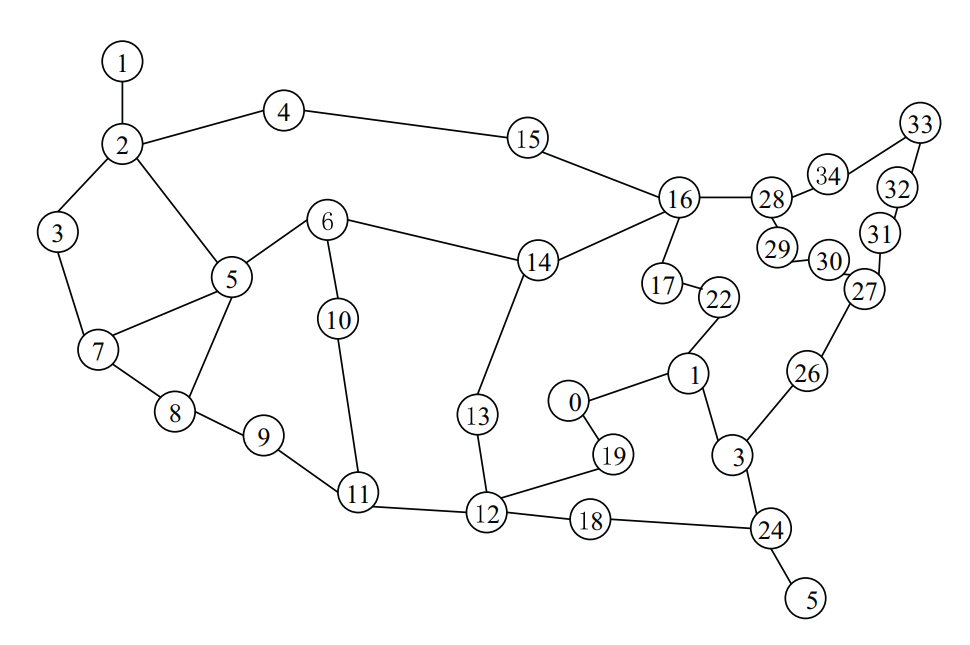
\includegraphics[width=\linewidth]{OS3E.png}
		\caption{Figure for Scenario 1}
		\label{fig:os3e}
	\end{figure}
	\begin{table}
		\caption{SPICi variations for Scenario 1}
		\begin{center}
			\begin{tabular}{|l|c|c|c|c|c|}
				\hline
				\textbf{Algorithm} & \textbf{$k$} & $\pi^{avgd}$ & \textbf{$\pi^{md}$} & \textbf{$\pi^{ic}$} & \textbf{$\pi^{latency}$} \\
				\hline
				SPICi & 14 & 1.1 & 2 & 4.12 & 7.22 \\
				Greedy & 7 & 1.44 & 3 & 4.33 & 8.78 \\
				V2($T_c=.45$) & 3 & 2.71 & 6 & 3.67 & 12.38 \\
				V3($T_c=.45$) & 3 & 2.45 & 6 & 5 & 13.45 \\
				V4($T_c=.45$) & 3 & 3.52 & 7 & 3 & 13.52 \\
				V2($T_c=.5$) & 9 & 1.44 & 3 & 4.47 & 8.91 \\
				V3($T_c=.$5) & 6 & 1.6 & 2 & 4.73 & 8.33 \\
				V4($T_c=.5$) & 6 & 2.68 & 4 & 5.13 & 11.81 \\
				Inverse($T_c=1.08$) & 4 & 3.29 & 6 & 5.33 & 14.62 \\
				\hline
			\end{tabular}
		\end{center}
		\caption{Final Comparison for Scenario 1}
		\begin{center}
			\begin{tabular}{|l|c|c|c|c|c|c|}
				\hline
				\textbf{Algorithm} & \textbf{$k$} & $\pi^{avgd}$ & \textbf{$\pi^{md}$} & \textbf{$\pi^{ic}$} & \textbf{$\pi^{latency}$} & \textbf{$|S|$} \\
				\hline
				DBCP & 5 & 1.45 & 3 & 4.2 & 8.65 & 9 \\
				DBCP-w & 5 & 1.45 & 3 & 4.2 & 8.65 & 9 \\
				SPICi & 14 & 1.1 & 2 & 4.12 & 7.22 & 3 \\
				G-SPICi & 7 & 1.44 & 3 & 4.33 & 8.78 & 7  \\
				SPICi-V3 & 6 & 1.6 & 2 & 4.73 & 8.33 & 7 \\
				I-SPICi & 4 & 3.29 & 6 & 5.33 & 14.62 & 9 \\
				\hline
			\end{tabular}
		\end{center}
	\end{table}

	
	Observing the data from the table we can understand that SPICi generates a lot of controllers for a greater network with more connectivity. Greedy somewhat reduces it but latency increases slightly. The variations of SPICi give different numbers of controllers based on the value of the threshold $T_c$.
	
	
	As mentioned earlier SPICi gives a huge number of controllers due to creation of isolated nodes. This happens because it creates clusters with nodes that are far away  and is noticeable specially in cases where highly connected and large number of nodes are present as in figure \ref{fig:os3e}. DBCP creates the optimum number of controllers and also selects cluster heads properly as the graph is unweighted.
	
	\subsubsection{Scenario 2}
	This is the SPICi dataset containing less nodes with greater proximity and similar weight edges. The edge weights are in the continuous range $(0,1)$. It is shown in the figure \ref{fig:spici}.
	\begin{figure}
		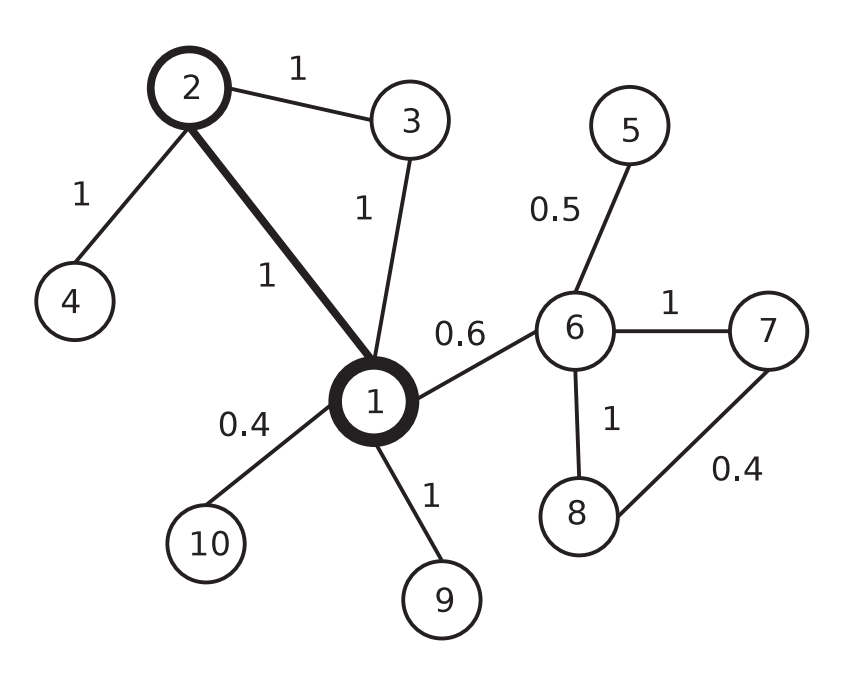
\includegraphics[width=\linewidth]{Spici.png}
		\caption{Figure for Scenario 2}
		\label{fig:spici}
	\end{figure}
	\begin{table}
		\caption{SPICi variations for Scenario 2}
		\begin{center}
			\begin{tabular}{|l|c|c|c|c|c|}
				\hline
				\textbf{Algorithm} & \textbf{$k$} & $\pi^{avgd}$ & \textbf{$\pi^{md}$} & \textbf{$\pi^{ic}$} & \textbf{$\pi^{latency}$} \\
				\hline
				SPICi & 6 & 1 & 1 & 1.62 & 3.62 \\
				Greedy & 6 & 1 & 1 & 1.62 & 3.62 \\
				V2($T_c=.5$) & 4 & 0.92 & 1 & 1.5 & 3.42 \\
				V3($T_c=.5$) & 2 & 1.32 & 2 & 0.6 & 3.92 \\
				V4($T_c=.5$) & 1 & 1.48 & 2 & 0 & 3.48 \\
				Inverse($T_c=1.01$) & 3 & 1.28 & 2 & 2 & 5.28 \\
				\hline
			\end{tabular}
		\end{center}
		\caption{Final Comparison for Scenario 2}
		\begin{center}
			\begin{tabular}{|l|c|c|c|c|c|c|}
				\hline
				\textbf{Algorithm} & \textbf{$k$} & $\pi^{avgd}$ & \textbf{$\pi^{md}$} & \textbf{$\pi^{ic}$} & \textbf{$\pi^{latency}$} & \textbf{$|S|$} \\
				\hline
				DBCP & 1 & 1.44 & 2 & N/A & 3.14 & 10 \\
				DBCP-w & 2 & 0.99 & 2 & 0.6 & 3.59 & 6 \\
				SPICi & 6 & 1 & 1 & 1.62 & 3.62 & 3 \\
				G-SPICi & 6 & 1 & 1 & 1.62 & 3.62 & 3 \\
				SPICi-V4 & 1 & 1.48 & 2 & 0 & 3.48 & 10 \\
				I-SPICi & 3 & 1.28 & 2 & 2 & 5.28 & 5 \\
				\hline
			\end{tabular}
		\end{center}
	\end{table}

	In this network there are smaller number of nodes and thus SPICi performs better but still with more controllers than required. We can understand that clearly from Table 3. The Greedy-SPICi gives the same result as SPICi as there is minimum change between them but the variations of SPICi give much better results. The Inverse-SPICi also gives better result but it can be improved if the $T_c$ threshold is tuned.
	DBCP and Modified-DBCP (DBCP-w) give the same results as the graph is small. DBCP shows better results in large graphs and DBCP-w maintains the same even if the edge weights vary greatly.
	
	\subsubsection{Scenario 3}
	This is a dataset we created with nodes at greater distances and few creating closely connected zones. The graph is depicted in figure \ref{fig:separate}. SPICi could not be applied as it uses weights smaller than or equal to 1.
	\begin{figure}
		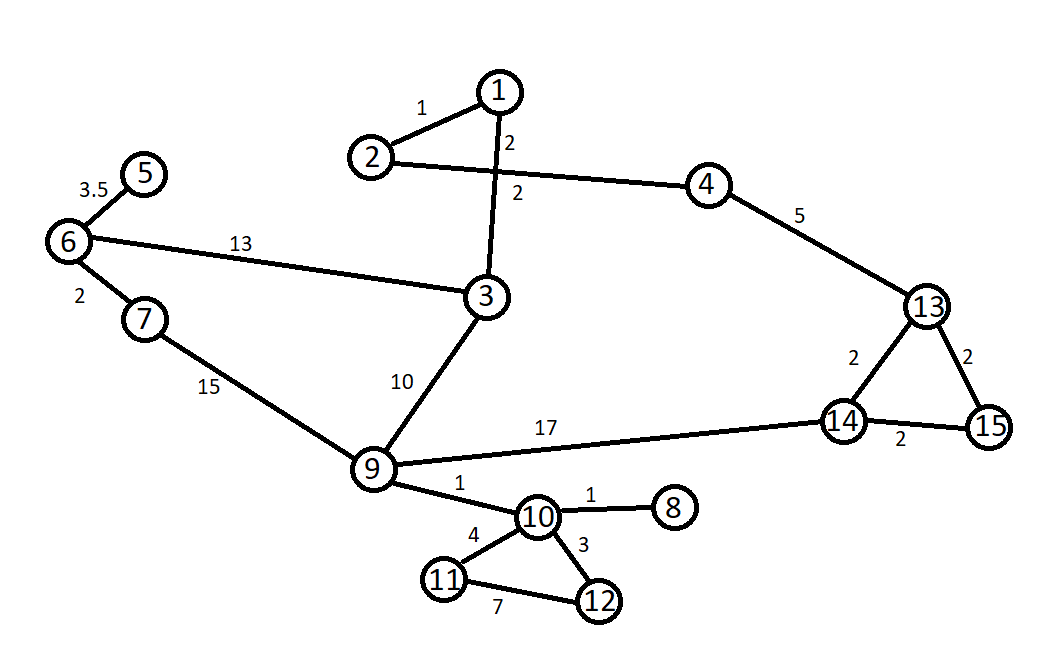
\includegraphics[width=\linewidth]{separated.png}
		\caption{Figure for Scenario 3}
		\label{fig:separate}
	\end{figure}
	\begin{table}
		\caption{SPICi variations for Scenario 3}
		\begin{center}
			\begin{tabular}{|l|c|c|c|c|c|}
				\hline
				\textbf{Algorithm} & \textbf{$k$} & $\pi^{avgd}$ & \textbf{$\pi^{md}$} & \textbf{$\pi^{ic}$} & \textbf{$\pi^{latency}$} \\
				\hline
				Greedy & 9 & 7.83 & 17 & 15.86 & 40.69 \\
				V2($T_c=.5$) & 4 & 9.59 & 20.5 & 15 & 45.09 \\
				V3($T_c=.5$) & 3 & 8.59 & 34 & 17.33 & 59.92 \\
				V4($T_c=.5$) & 3 & 10.32 & 27 & 9.33 & 46.65 \\
				Inverse & 5 & 5.79 & 15 & 16.8 & 37.59 \\
				\hline
			\end{tabular}
		\end{center}
		\caption{Final Comparisons for Scenario 3}
		\begin{center}
			\begin{tabular}{|l|c|c|c|c|c|c|}
				\hline
				\textbf{Algorithm} & \textbf{$k$} & $\pi^{avgd}$ & \textbf{$\pi^{md}$} & \textbf{$\pi^{ic}$} & \textbf{$\pi^{latency}$} & \textbf{$|S|$} \\
				\hline
				DBCP & 2 & 11.89 & 20.5 & 15 & 47.39 & 14 \\
				DBCP-w & 6 & 2.83 & 7 & 13.67 & 23.5 & 5 \\
				G-SPICi & 9 & 7.83 & 17 & 15.86 & 40.69 & 3 \\
				SPICi-V2 & 4 & 9.59 & 20.5 & 15 & 45.09 & 6 \\
				I-SPICi & 5 & 5.79 & 15 & 16.8 & 37.58571 & 4 \\
				\hline
			\end{tabular}
		\end{center}
	\end{table}
	
	As expected SPICi and DBCP both give unsatisfactory results as the edges have weights of greater variations. For greater weights SPICi takes nodes with greater weighted degree without considering it's distance from the controller. Instead it takes the farthest node first. DBCP also ignores the edge weights and takes each edge as one hop so this increases the controller to node distances. But in this case DBCP-w clusters the network better. I-SPICi also performs better than the other SPICi variations.

\end{document}